\documentclass[slovene,11pt,a4paper]{article}
\usepackage[margin=2cm,bottom=3cm,foot=1.5cm]{geometry}
% \documentclass[slovene,11pt,a4paper]{article}
% \usepackage[margin=1.7cm,bottom=3cm,foot=1.5cm]{geometry}
\setlength{\parindent}{0pt}
\setlength{\parskip}{0.5ex}

\usepackage[pdftex]{graphicx}
\usepackage{pgffor}
\usepackage{subcaption}
% \usepackage{a4wide} %najaci package
\usepackage[utf8]{inputenc}
\usepackage[slovene]{babel}
\usepackage{color}
\usepackage{graphicx}
% \usepackage{subfigure}
\usepackage{imakeidx}
\usepackage{adjustbox}
\usepackage{float}
\usepackage{amsmath}
\usepackage{mathtools}
\usepackage{tikz}
\usepackage{amssymb}
\usepackage{listings}
\usepackage{siunitx}
\usepackage{hyperref}
\usepackage{amsfonts}
\usepackage{mathrsfs}



\def\phi{\varphi}
\def\eps{\varepsilon}
\def\theta{\vartheta}

\newcommand{\thisyear}{2024/25}

\renewcommand{\Re}{\mathop{\rm Re}\nolimits}
\renewcommand{\Im}{\mathop{\rm Im}\nolimits}
\newcommand{\Tr}{\mathop{\rm Tr}\nolimits}
\newcommand{\diag}{\mathop{\rm diag}\nolimits}
\newcommand{\dd}{\,\mathrm{d}}
\newcommand{\ddd}{\mathrm{d}}
\newcommand{\ii}{\mathrm{i}}
\newcommand{\lag}{\mathcal{L}\!}
\newcommand{\ham}{\mathcal{H}\!}
\newcommand{\four}[1]{\mathcal{F}\!\left(#1\right)}
\newcommand{\bigO}[1]{\mathcal{O}\!\left(#1\right)}
\newcommand{\sh}{\mathop{\rm sinh}\nolimits}
\newcommand{\ch}{\mathop{\rm cosh}\nolimits}
\renewcommand{\th}{\mathop{\rm tanh}\nolimits}
\newcommand{\erf}{\mathop{\rm erf}\nolimits}
\newcommand{\erfc}{\mathop{\rm erfc}\nolimits}
\newcommand{\sinc}{\mathop{\rm sinc}\nolimits}
\newcommand{\rect}{\mathop{\rm rect}\nolimits}
\newcommand{\ee}[1]{\cdot 10^{#1}}
\newcommand{\inv}[1]{\left(#1\right)^{-1}}
\newcommand{\invf}[1]{\frac{1}{#1}}
\newcommand{\sqr}[1]{\left(#1\right)^2}
\newcommand{\half}{\frac{1}{2}}
\newcommand{\thalf}{\tfrac{1}{2}}
\newcommand{\pd}{\partial}
\newcommand{\Dd}[3][{}]{\frac{\ddd^{#1} #2}{\ddd #3^{#1}}}
\newcommand{\Pd}[3][{}]{\frac{\pd^{#1} #2}{\pd #3^{#1}}}
\newcommand{\avg}[1]{\left\langle#1\right\rangle}
\newcommand{\norm}[1]{\left\Vert #1 \right\Vert}
\newcommand{\braket}[2]{\left\langle #1 \vert#2 \right\rangle}
\newcommand{\obraket}[3]{\left\langle #1 \vert #2 \vert #3 \right \rangle}
\newcommand{\hex}[1]{\texttt{0x#1}}

\renewcommand{\iint}{\mathop{\int\mkern-13mu\int}}
\renewcommand{\iiint}{\mathop{\int\mkern-13mu\int\mkern-13mu\int}}
\newcommand{\oiint}{\mathop{{\int\mkern-15mu\int}\mkern-21mu\raisebox{0.3ex}{$\bigcirc$}}}

\newcommand{\wunderbrace}[2]{\vphantom{#1}\smash{\underbrace{#1}_{#2}}}

\renewcommand{\vec}[1]{\overset{\smash{\hbox{\raise -0.42ex\hbox{$\scriptscriptstyle\rightharpoonup$}}}}{#1}}
\newcommand{\bec}[1]{\mathbf{#1}}


\title{
\sc\large Matematično-fizikalni praktikum \thisyear\\
\bigskip
\bf\Large 6.~naloga: Enačbe hoda
}
\author{Tadej Tomažič}
\date{}

\makeindex[columns=3, title=Alphabetical Index, intoc]

\begin{document}


\pagenumbering{gobble} 
\author{Tadej Tomažič}
\date{\today}

\maketitle

\newpage
\pagenumbering{arabic}
\tableofcontents
\listoffigures
\newpage
\section{Navodila}



Za opis najpreprostejših fizikalnih procesov uporabljamo
navadne diferencialne enačbe, ki povezujejo vrednosti
spremenljivk sistema z njihovimi časovnimi
spremembami. Tak primer je na primer enačba za časovno
odvisnost temperature v stanovanju, ki je obdano s stenami
z neko toplotno prevodnostjo in določeno zunanjo temperaturo.
V najpreprostejšem primeru ima enačba obliko
\begin{equation}
\Dd{T}{t} = - k \left( T-T_\mathrm{zun} \right)
\label{cooling}
\end{equation}
z analitično rešitvijo
\begin{equation*}
T(t) = T_\mathrm{zun} + \mathrm{e}^{-kt} \left( T(0) - T_\mathrm{zun} \right) \>.
\end{equation*}
Enačbam, ki opisujejo razvoj spremenljivk sistema $y$ po času ali drugi
neodvisni spremenljivki $x$, pravimo {\sl enačbe hoda\/}.  Pri tej
nalogi bomo proučili uporabnost različnih numeričnih metod
za reševanje enačbe hoda oblike $\ddd y/\ddd x = f(x, y)$,
kot na primer~(\ref{cooling}).   Najbolj groba
prva inačica, tako imenovana osnovna Eulerjeva metoda,
je le prepisana aproksimacija za prvi odvod
$y' \approx (y(x+h) - y(x)) / h$, torej
\begin{equation}
y(x+h) = y(x) + h\,\left.\Dd{y}{x}\right|_x \>.
\label{euler}
\end{equation}
Diferencialno enačbo smo prepisali
v diferenčno: sistem
spremljamo v ekvidistantnih korakih dolžine $h$. Metoda je
večinoma stabilna, le groba: za večjo natančnost moramo
ustrezno zmanjšati korak.   Za red boljša (${\cal O}\,(h^3 )$ , t.j. lokalna natančnost drugega reda)
je simetrizirana Eulerjeva (ali sredinska) formula, ki sledi
iz simetriziranega približka za prvi odvod,
$y' \approx (y(x+h) - y(x-h)) / 2h$.  Računamo po shemi
\begin{equation}
y(x+h) = y(x-h) + 2h\,\left.\Dd{y}{x}\right|_x \>,
\label{seuler}
\end{equation}
ki pa je praviloma nestabilna.  Želeli bi si
pravzaprav nekaj takega
\begin{equation}
y(x+h) = y(x) + {h\over 2}\,\left[\left.\Dd{y}{x}\right|_x
+ \left.\Dd{y}{x}\right|_{x+h} \right] \>,
\label{impeuler}
\end{equation}
le da to pot ne poznamo odvoda v končni točki intervala
(shema je implicitna). Pomagamo si lahko z iteracijo.
Zapi\v simo odvod kot:
$$ \left.{dy \over dx}\right|_x = f(x,y) $$ ter $$ x_{n+1} = x_n + h,
~~~ y_n = y(x_n)$$
Heunova metoda (${\cal O}\,(h^3 )$ lokalno) je pribli\v zek idealne formule z:
\begin{eqnarray}
\hat{y}_{n+1} & =  & y_n +  h \cdot f(x_n,y_n) \\
y_{n+1} & = & y_n + \frac{h}{2} \left[ f(x_n,y_n) + f(x_{n+1},\hat{y}_{n+1})\right]
\end{eqnarray}
Izvedenka tega je nato Midpoint metoda  (tudi ${\cal O}\,(h^3 )$ lokalno):
\begin{eqnarray}
k_1 & = & f(x_n,y_n) \\
k_2 & = & f(x_n+{1 \over 2}h,y_n+{1 \over 2}\, h\,k_1) \\
y_{n+1} & = & y_n + h\,k_2
\end{eqnarray}
Le-to lahko potem izbolj\v samo kot modificirano Midpoint metodo
itd\ldots

V praksi zahtevamo natančnost in numerično učinkovitost,
ki sta neprimerno boljši kot pri opisanih preprostih metodah.
Uporabimo metode, zasnovane na algoritmih prediktor-korektor,
metode višjih redov iz družine Runge-Kutta (z adaptivnimi koraki), ali ekstrapolacijske metode.
Brez dvoma ena najbolj priljubljenih je metoda RK4,
\begin{align}
k_1 & =
  f\left(x,\,{y}(x)\right) \> {,}\nonumber\\
k_2 & =
  f\left(x+{\textstyle{1\over 2}}h,\,
       {y}(x)+{\textstyle{h\over 2}}k_1\right) \> {,}\nonumber\\
k_3 & =
  f\left(x+{\textstyle{1\over 2}}h,\,
       {y}(x)+{\textstyle{h\over 2}}k_2\right) \> {,}\label{eq:rk4}\\
k_4 & =  f\left(x+h,\,{y}(x)+hk_3\right) \> {,}\nonumber\\
{y}(x+h) & =  {y}(x)
  + {\tfrac{h}{6}}\,\left(k_1 + 2k_2 + 2k_3 + k_4\right) + {\cal O}(h^5)
  \nonumber\> {.}
\end{align}

\bigskip

{\it Naloga\/}: preizkusi preprosto Eulerjevo metodo ter nato še čim več 
naprednejših metod( Midpoint, Runge-Kutto 4. reda, Adams-Bashfort-Moultonov prediktor-korektor \ldots ) na primeru
z začetnima temperaturama $y(0)=21$ ali $y(0)=-15$,
zunanjo temperaturo $y_\mathrm{zun}=-5$ in parametrom $k=0.1$.
Kako velik (ali majhen) korak $h$ je potreben?
Izberi metodo (in korak) za izračun družine rešitev
pri različnih vrednostih parametra $k$.

\bigskip

{\it Dodatna naloga\/:} temperatura prostora se lahko še
dodatno spreminja zaradi denimo sončevega segrevanja
skozi okna, s $24$-urno periodo in nekim faznim zamikom $\delta$,
kar opišemo z dva- ali triparametrično enačbo
\begin{equation}
\Dd{T}{t} = - k \left( T-T_\mathrm{zun} \right)
+ A\sin\left( {2\pi\over 24}(t-\delta) \right) \>.
\label{cooling2}
\end{equation}
Poišči še družino rešitev te enačbe pri
$k=0.1$ in $\delta=10$!  Začni z $A=1$, kasneje spreminjaj tudi
to vrednost.  V premislek: kakšno metodo bi uporabil, če bi posebej
natančno želel določiti maksimalne temperature in trenutke,
ko nastopijo?

\section{Rešitev}

Najprej si poglejmo avtokorelacijo za obe sovi.
\begin{figure}[h]
    \centering
    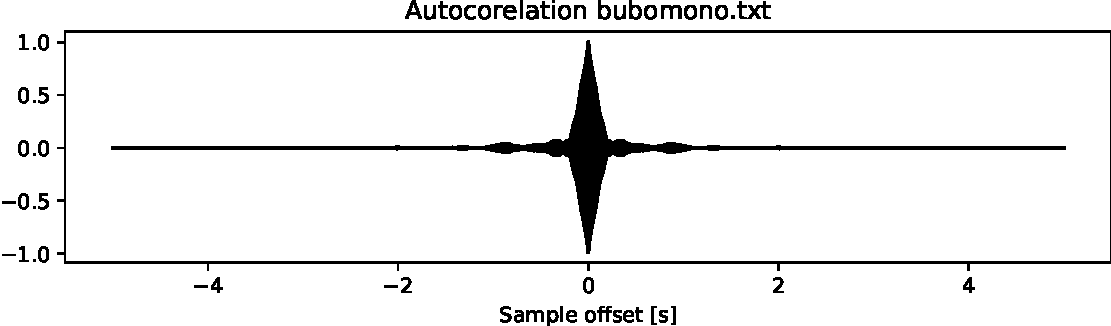
\includegraphics[width=12cm]{pdfs/bubomono.txt_acor.pdf}
    \vspace{10pt}
    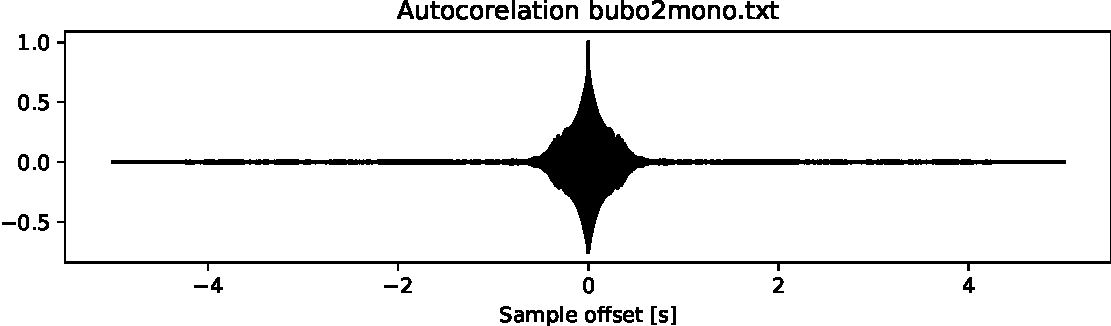
\includegraphics[width=12cm]{pdfs/bubo2mono.txt_acor.pdf}
    \caption{Avtokorelacija signala sov}
\end{figure}

Preden sem koreliral signal sem vektorja samplov normiral, tako da je
"najmočnejši" signal 1. To pomeni \[\|x\|_\infty = \max_i |x_i|\]

Poglejmo si še korelacije med sovami in posnetki:
\newpage
\begin{figure}[h]
    \centering
    \foreach \mix in {mix, mix1, mix2, mix22} {
        \foreach \sova in {bubomono, bubo2mono}{
            \includegraphics[width=8cm]{pdfs/cor_\mix.txt_\sova.txt.pdf}
        }
    }
    \caption{Korelacija sov in posnetkov iz narave}
\end{figure}
Tukaj je bila normalizacija drugače izbrana. Tukaj je bila narejena normalizacija korelacije. Če je varianca signala a $\sigma_a$,
potem je $ \mathbf{x} = \mathbf{x} / \left(\sigma_a \sigma_b |\mathbf{b}|\right)$. Sigma je izračunana z \verb|numpy.std()|.


Hitrosti so precej dolgčasno pričakovane ampak vseeno.
\begin{figure}[h]
    \centering
    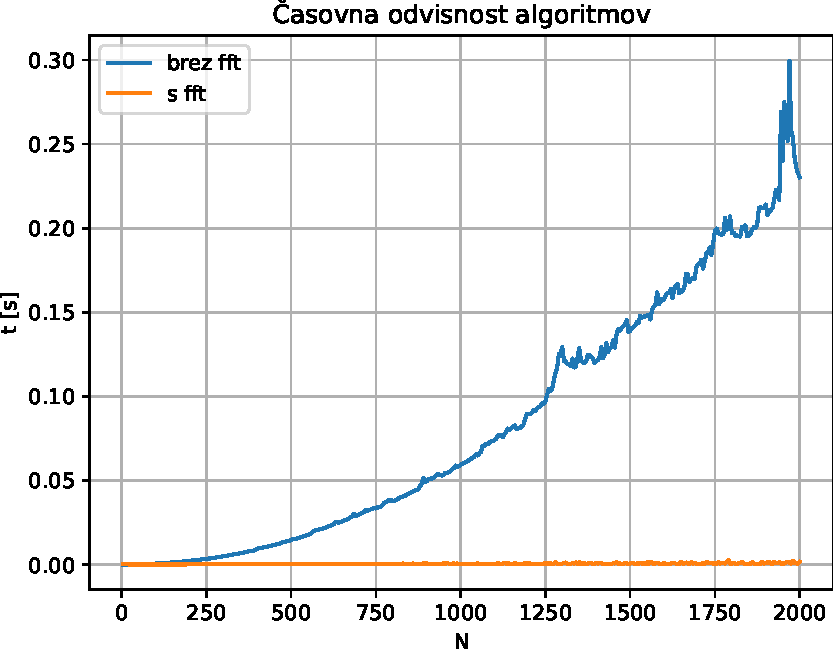
\includegraphics[width=8cm]{pdfs/cas-lin.pdf}
    \vspace{10pt}
    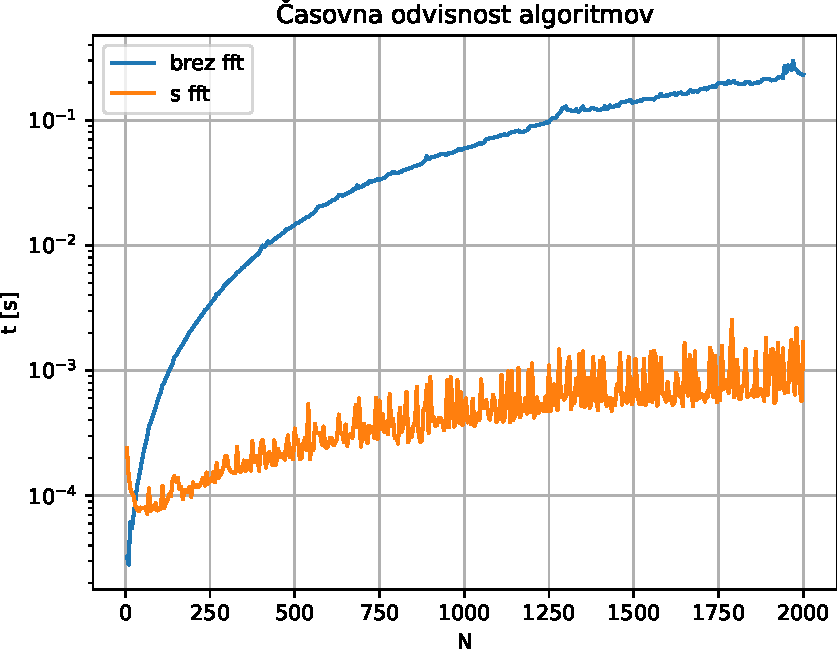
\includegraphics[width=8cm]{pdfs/cas-log.pdf}
    \caption{Hitrost algoritmov}
\end{figure}
\newpage
\section{Dodatna naloga}
Posnel sem dva človeka m in ž ko izgovarjata aaaaaaaaaaaa. Posnel sem jih tudi
ko bereta slovar. Gledal sem ali lahko spet zaznam ali gre za ž glas ali m glas.
Poglejmo si spektra njunega glasu.
\begin{figure}[h]
    \begin{center}
        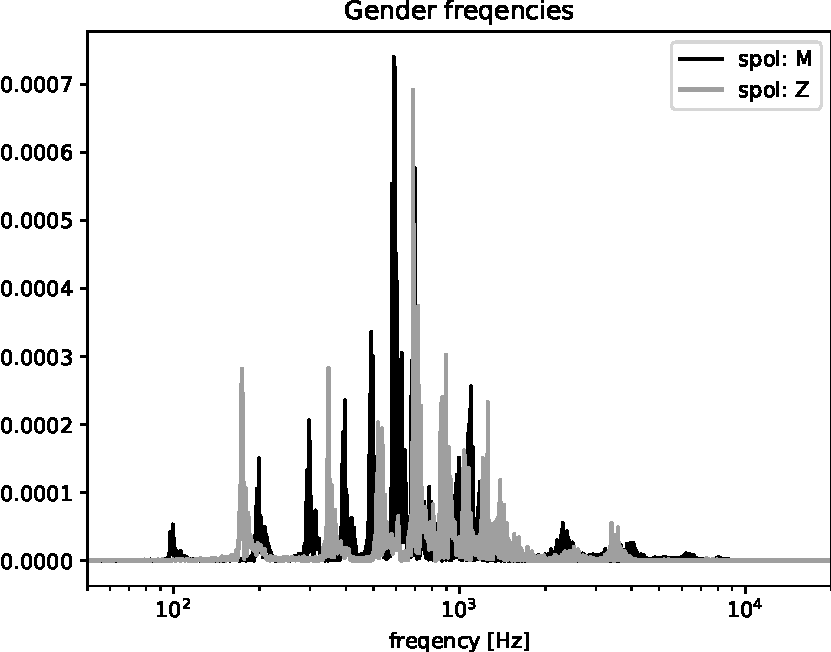
\includegraphics[width=12cm]{pdfs/fft_spol.pdf}
    \end{center}
    \caption{Barva glasu moškega in ženske}
\end{figure}

% Glasova sta bila prej normirana, saj je bil moški glas posnet bližje mikrofona.
% Poglejmo si zopet korelacijo med posnetki:
% \foreach \gender in {Z, M} {
%     \foreach \mix in {Glas\ 001, Glas\ 002}{
%         pdfs/cor_\gender_\mix.pdf 
%     }
% }
\begin{figure}[h]
    \begin{center}
        
    \foreach \gender in {Z, M} {%
        \foreach \mix in {001, 002} {%
            \includegraphics[width=8cm]{pdfs/cor_\gender_Glas\space\mix.pdf}%    
        }%
        \par
}%
    \end{center}
    
    \caption{Korelacija glasa človeka in posnetkov iz branja slovarja}
\end{figure}
\end{document}
